\documentclass[a4paper]{article}

%% Language and font encodings
\usepackage[english]{babel}
\usepackage[utf8x]{inputenc}
\usepackage[T1]{fontenc}

%% Sets page size and margins
\usepackage[a4paper,top=3cm,bottom=2cm,left=3cm,right=3cm,marginparwidth=1.75cm]{geometry}

%% Useful packages
\usepackage{amsmath}
\usepackage{graphicx}
\usepackage[colorinlistoftodos]{todonotes}
\usepackage[colorlinks=true, allcolors=blue]{hyperref}

% \usepackage{xltxtra}
\usepackage{rotating,makecell}
\usepackage{dcolumn}
\usepackage{upgreek}
% \usepackage{amssymb}
\usepackage{multirow, booktabs}
\usepackage{siunitx}

\title{Analysis Note: \\
Measurement of $D^0$-meson production in Au+Au collisions at $\sqrt{s_{\rm NN}}$ = 200\,GeV}
\author{Xiaolong Chen, Xin Dong, Mustafa Mustafa, Guannan Xie, Yifei Zhang, Long Zhou}

\begin{document}
\maketitle

\begin{abstract}

Heavy quarks nuclear modification factor ($R_{AA}$) has been proposed as an important measurement to study the flavor dependence of partons energy loss in the medium, and eventually to help in extracting the medium transport, drag and diffusion coefficients.

We report the first measurement of efficiency corrected spectrum for $D^0$ from HFT through the hadronic channels ($D^0(\bar{D^0}) \rightarrow K^{\mp}\pi^{\pm}$), the Nuclear Modification Factor ($R_{AA}$) of $D^0$ mesons in Au+Au collisions at $\sqrt{s_{NN}}$ = 200 GeV. The precision was much better compared to previous published one. The new $R_{AA}$ results show significant suppression at high $p_T$ which means the strong interaction between charm quark and the medium and loose energy. While the $D^0$ $R_{AA}$ shows quite similar trend as light hadrons.

\end{abstract}

\section{Introduction}

Heavy quarks nuclear modification factor ($R_{AA}$) has been proposed as an important measurement to study the flavor dependence of partons energy loss in the medium, and eventually to help in extracting the medium transport, drag and diffusion coefficients. There are lots of theoretical calculations for the energy losses for different flavor particles. Fig.~\ref{fig:raa_CUJE} shows the jet flavor tomography level crossing pattern of nuclear modification factors at middle rapidity of $\pi$, D, B, e from CUJT calculations for central Au + Au 200 GeV collisions. As clearly see the mass hierarchy of the different flavor energy loss.

\begin{figure}
\centering
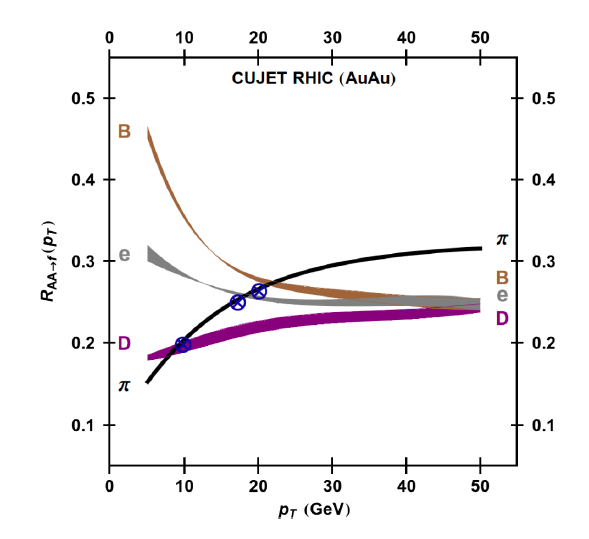
\includegraphics[width=0.5\textwidth]{fig/raa_CUJE.png}
\caption{Jet flavor tomography level crossing pattern of nuclear modification factors at middle rapidity of $\pi$, D, B, e calculations for central Au + Au 200 GeV collisions.}
\label{fig:raa_CUJE} 
\end{figure}

The hadronic channels allow to fully reconstruct the charmed hadrons and do not suffer from the complications in the semi-leptonic decays, however the measurement can be challenging due to large combinatorial backgrounds and lower branching ratios. One approach is to use the decay topology to reduce this background by distinguishing between tracks that come from the collision itself (primary vertex) and those from a secondary decay vertex. This requires the detectors must be able to resolve differences on the order of tens of microns. Heavy Flavor Tracker (HFT) is essence the right detector for this mission.

Fig.~\ref{fig:BeforeHFT} shows the $R_{AA}$ of $D^0$, $\pi$, $h^{\pm}$ from various measurements. A significant suppression is clearly seen at the high $p_T$ range for both light hadrons and charmed hadrons both in RHIC energy and LHC energy. The enhancement observed in the intermediate $p_T$ range from STAR can be described by the models including coalescence of charm and light quarks, even though the uncertainties are still large in the low transverse momentum range. It will be critical to precise measure the low $p_T$ structure.

\begin{figure}
\centering
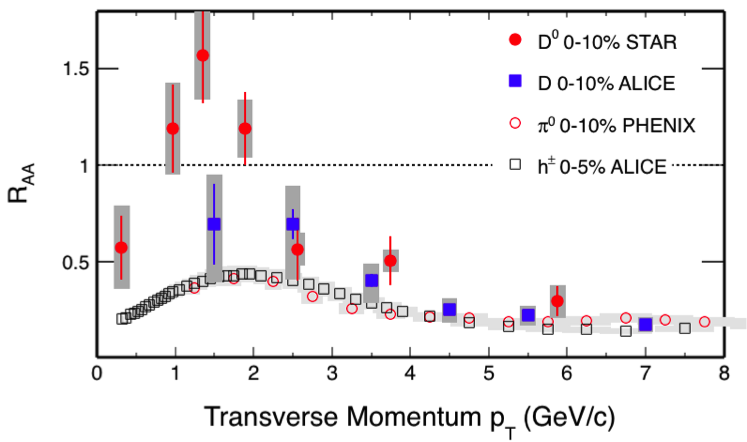
\includegraphics[width=0.5\textwidth]{fig/BeforeHFT.png}
\caption{(upper) $D^0$, $\pi$, $h^{\pm}$ $R_{AA}$ from different measurements. (bottom) $v_2$ of $D$ and $h^{\pm}$ from ALICE.}
\label{fig:BeforeHFT} 
\end{figure}

\section{\label{dataset}Datasets and Event Selection}

The dataset used in this analysis is P16id production of 2014 Au+Au 200 GeV data. This is the first year of physics running the new STAR HFT Detector. The analysis uses picoDst which is produced from MuDst.

The Minimum-Bias (MinBias) trigger is defined as a coincidence between the two VPDs, and an online collision vertex cut. Moreover, a pile-up protection at the trigger level was applied for the data taking. In this analysis, the MinBias trigger, denoted as ``vpdmb-5-p-nobsmd" and ``vpdmb-5-p-nobsmd-hlt", is used. The triggers used in this analysis are listed in Table~\ref{trigger}.

\begin{table}[htp]
\centering
\caption{Triggers ID used in this analysis from run14}
\label{trigger}
	\begin{center}
	\begin{tabular}{l|l}
%  \Xhline{1.6pt}
	Trigger ID	& description\\ \hline
	450050		& vpdmb-5-p-nobsmd-hlt\\ \hline
	450060		& vpdmb-5-p-nobsmd-hlt\\ \hline
	450005		& vpdmb-5-p-nobsmd\\ \hline
	450015		& vpdmb-5-p-nobsmd\\ \hline
	450025		& vpdmb-5-p-nobsmd\\ \hline
%  \Xhline{1.6pt}
	\end{tabular}
	\end{center}
\end{table}

Events used in this analysis are required to have a valid collision vertex $V_{z}$ (primary vertex) within 6 cm of the TPC center along $z$ direction (the beam direction) to ensure a uniform TPC acceptance and make sure the most tracks are within the PiXeL (PXL) detector coverage. The PXL detector is about 20 cm along the z direction, and the radius of the inner layer is about 2.8cm and outer layer is about 8 cm. Furthermore, the distance between the $V_{z}$ constructed by TPC and the vertex constructed by VPD ($V_{z}^{VPD}$, fast detector) is within 3 cm to reject the bad events. A radial length less than 2 cm for the vertex is required to reject the events from the beam hitting the beam pipe. After event selection, $\sim$875 million MinBias events are used for this analysis. Table~\ref{eventselection} lists the event selection criterion.

\begin{table}[htp]
\centering
\caption{Event selection in Au+Au collisions at 200 GeV for $D^0$.}
\label{eventselection}
\begin{tabular}{c}
\toprule[1.6pt]
Event Selection Criteria \\
\midrule[1.2pt]
\multirow{2}*{$!(|V_{x}|== 0 \ \&\& \ |V_{y}|== 0 \  \&\& \  |V_{z}|== 0) $ } \\
\\
\multirow{2}*{$|V_{z}|<$ 6 cm} \\
\\
\multirow{2}*{$|V_{r}|<$ 2 cm} \\
\\
\multirow{2}*{$|V_{z} - V_{z}^{VPD}|<$ 3 cm} \\ 
\\  
\bottomrule[1.6pt]
\end{tabular}
\end{table}

\subsection{Centrality Definition}

The centrality for Run14 200GeV Au+Au collisions MinBias sample is based on gRefMult. The gRefMult is defined as the number of global tracks with $|\eta|<0.5$, no less than 10 TPC hits, and Distance of Closest Approach (DCA) to primary vertex less than 3 cm with some correction according to $V_{z}$ and luminosity. The centrality definition according to the corrected gRefMult is listed in Table ~\ref{fig:centrality}. This is decided by comparing the measured gRefMult distribution with the Glauber model simulation. 

The basic procedure for centrality definition have three steps. First, need the quality assurance (QA) for the data set and remove those outlier runs. The second step would be correct the $V_{z}$ and luminosity dependence for the reference multiplicity (gRefmult). The last step would be compare our data with Glauber MC simulation and determine the centrality classification.

For the QA, several variables are used for the outlier selection, such as Refmult (primary track multiplicity), gRefmult (global track multiplicity), TofRefmult (tof track multiplicity) and etc. In the Fig.~\ref{fig:centrality_QA1} shows the $\langle$gRefmult$\rangle$ as a function of run index for the QA, and there are several outliers are identified. Those dashed lines are the 4$\times$RMS range, beyond those range, the runs are identified as bad run. And several iterations are did until all the runs are within these 4$\times$RMS range.


In the Fig.~\ref{fig:centrality_QA2} shows the $\langle$HFT $p_{T}$$\rangle$, which is the mean $p_{T}$ of HFT tracks, as a function of run index for the QA, and we can clearly see there is a deep before the run index $\sim$520 which corresponding to the run number 15107008. And also we saw the same structure in the Fig.~\ref{fig:centrality_QA3}, which shows the average of HFT matching Ratio in the $p_{T}$ range between 0.7 to 0.8 GeV/$c$ and Fig.~\ref{fig:centrality_QA4} shows this HFT matching ratio in the high $p_{T}$ range. So, basically those runs before day 107 were taken out for this analysis, since it will complicate our efficiency calculation.

This deep was identified later on with a lot of effort, it was due to the firmware issue. And more details can be found in the STAR documents below.

\url{https://drupal.star.bnl.gov/STAR/system/files/STAR_PXL_Firmware_Issue_Solved_Final_Report_Oct3_v2.pdf}

\begin{figure}[htbp]
\begin{minipage}[htbp]{0.52\linewidth}
\centering
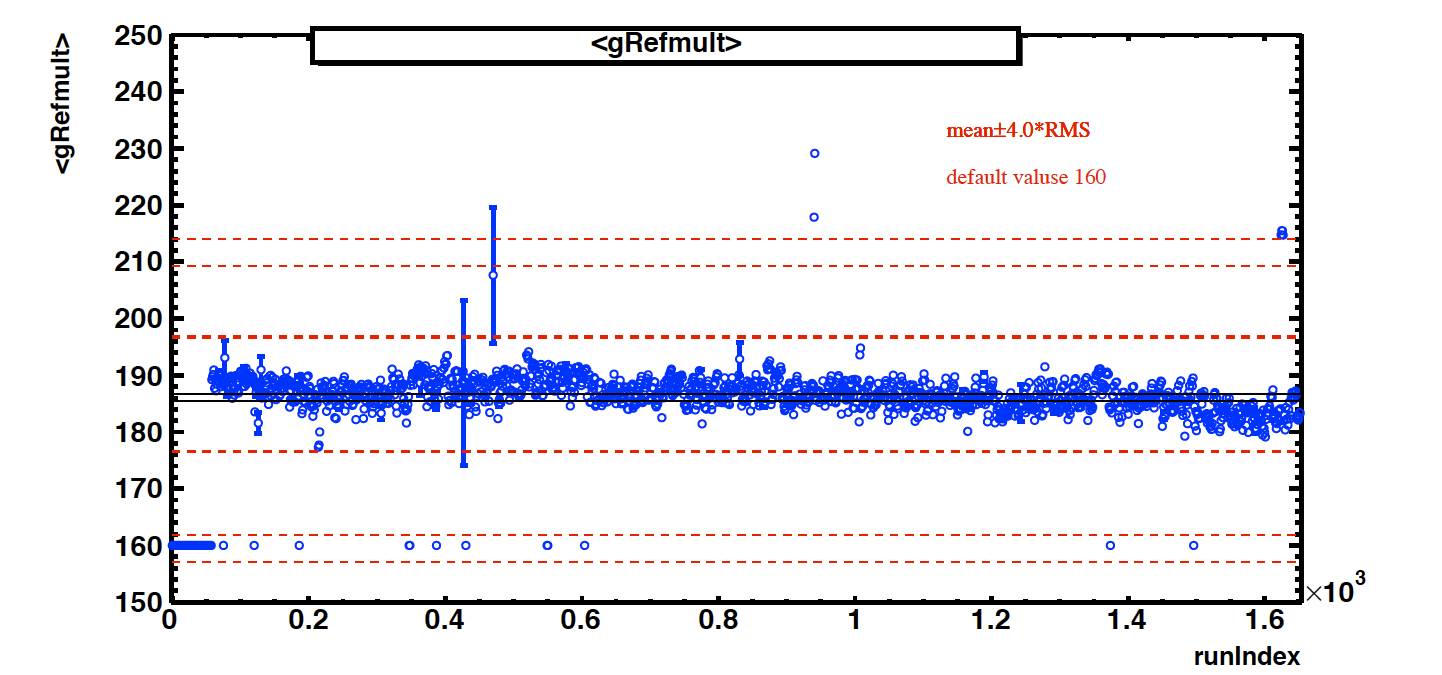
\includegraphics[width=1.0\textwidth]{fig/centrality_grefmult.png}
\caption{The mean value of gRefmult ($\langle$gRefmult$\rangle$) as a function of run index from QA.\label{fig:centrality_QA1}}
\end{minipage}
\hfill
\begin{minipage}[htbp]{0.52\linewidth}
\centering
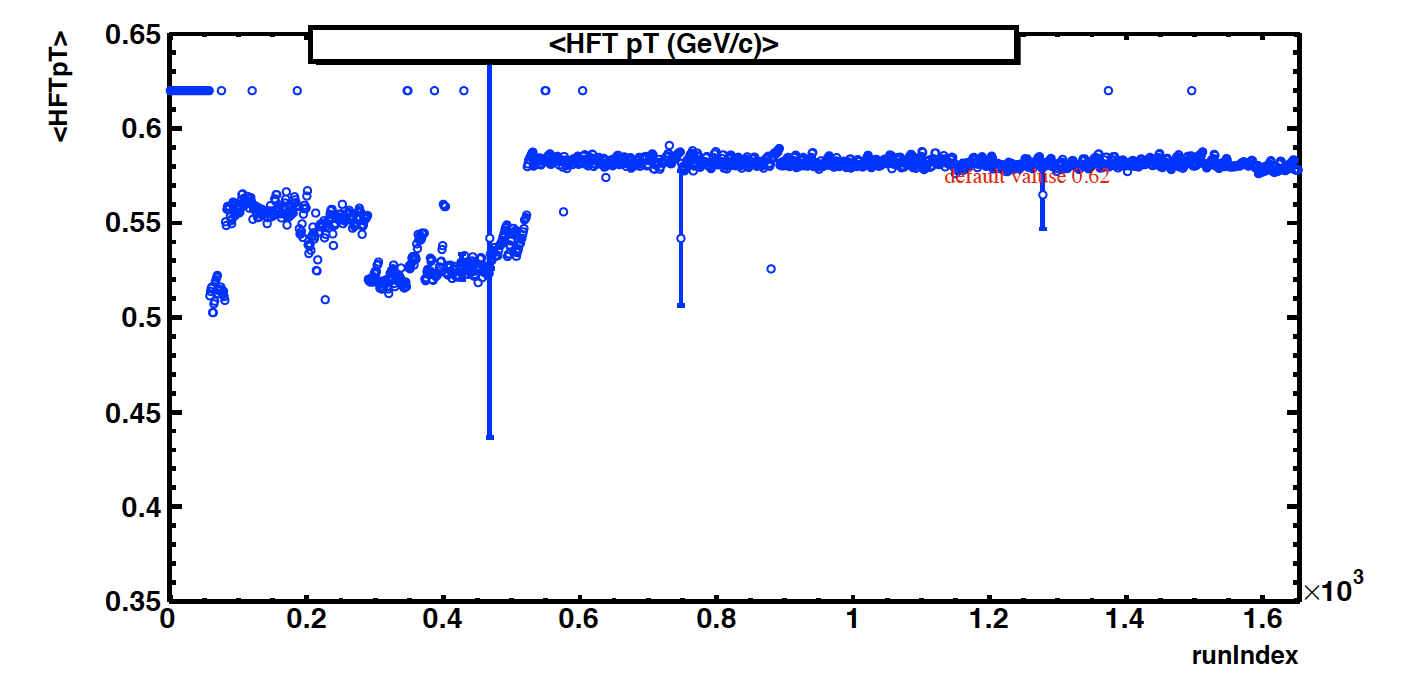
\includegraphics[width=1.0\textwidth]{fig/centrality_HFTpt.png} 
\caption{The mean value of $p_{T}$ for HFT matched track ($\langle$HFT $p_{T}$$\rangle$) as a function of index.\label{fig:centrality_QA2}}
\end{minipage}
\end{figure}


\begin{figure}[htbp]
\begin{minipage}[htbp]{0.52\linewidth}
\centering
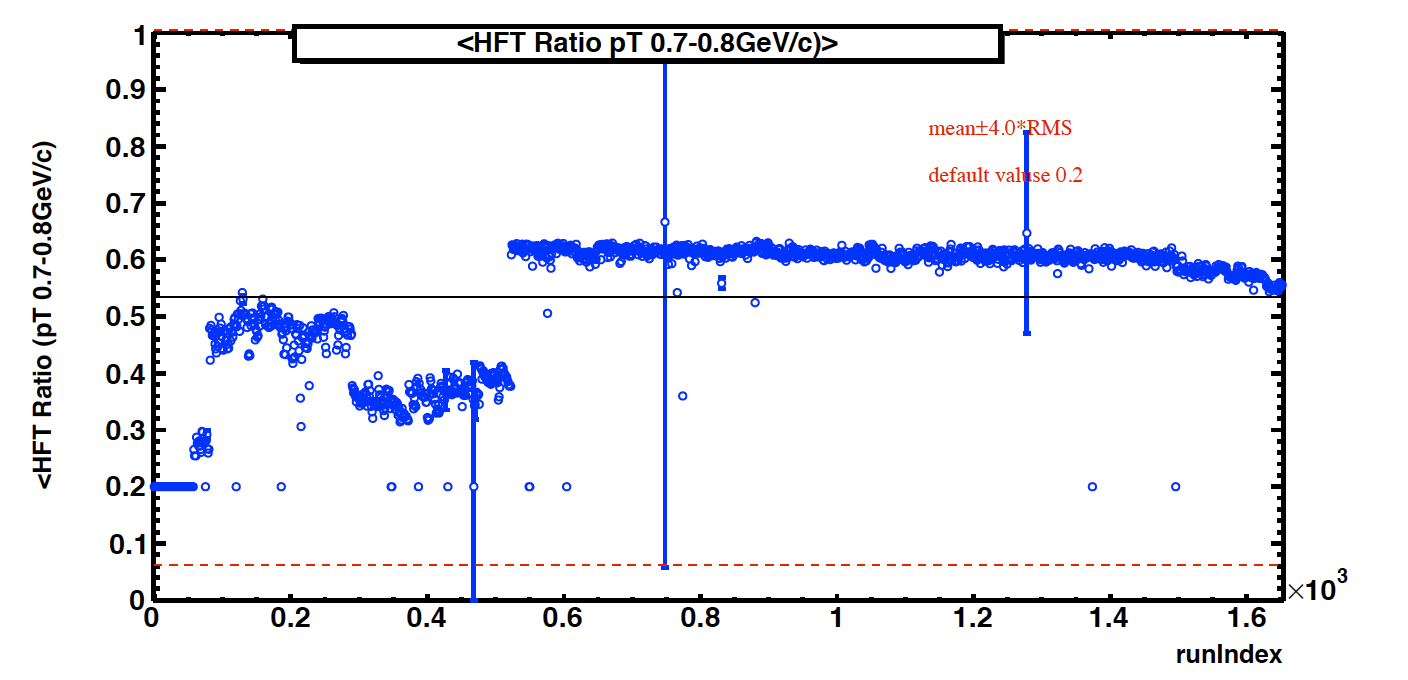
\includegraphics[width=1.0\textwidth]{fig/centrality_HFTratio.png}
\caption{The mean value of HFT matching ratio ($\langle$HFT $p_{T}$$\rangle$) as a function of run index at the transverse momentum range 0.7 < $p_{T}$ < 0.8 GeV/$c$.\label{fig:centrality_QA3}}
\end{minipage}
\hfill
\begin{minipage}[htbp]{0.52\linewidth}
\centering
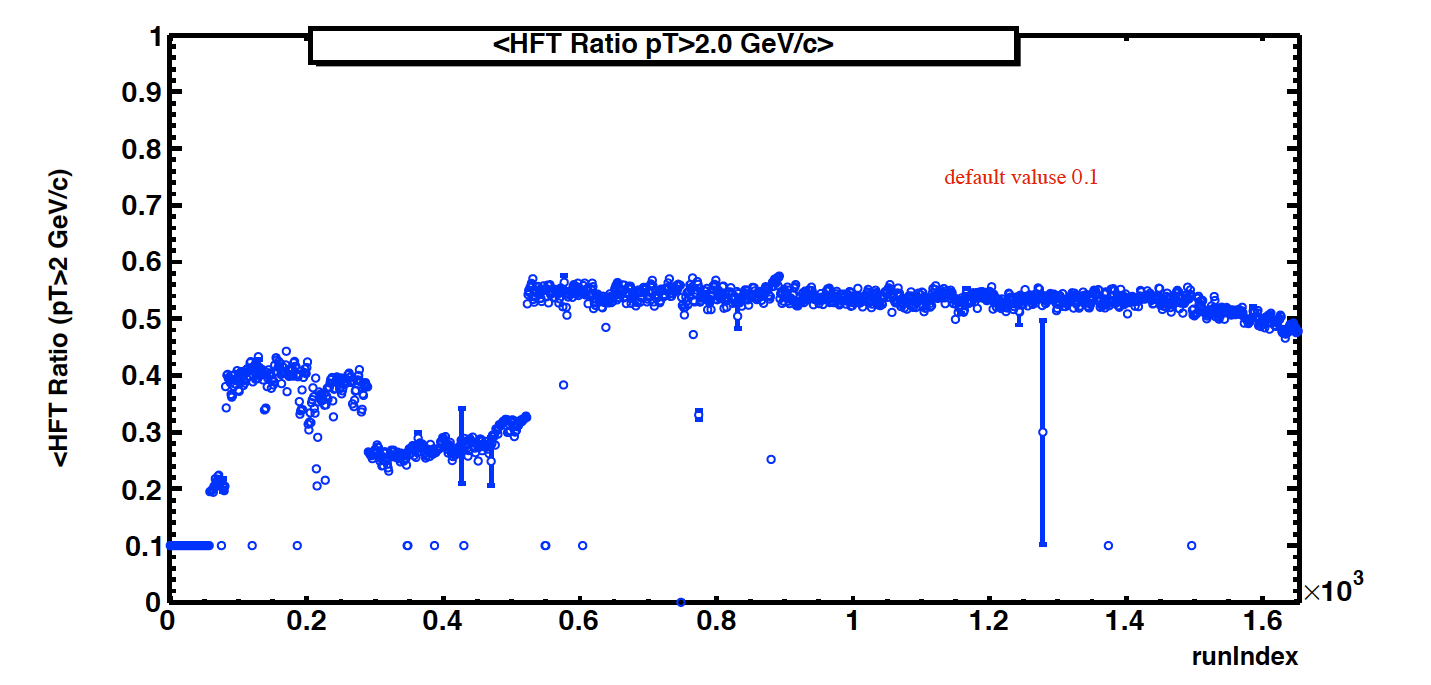
\includegraphics[width=1.0\textwidth]{fig/centrality_HFTratio2.png} 
\caption{The mean value of HFT matching ratio ($\langle$HFT $p_{T}$$\rangle$) as a function of run index at the transverse momenaum range $p_{T}$ > 2.0 GeV/$c$.\label{fig:centrality_QA4}}
\end{minipage}
\end{figure}

Fig.~\ref{fig:MB5_vz} and Fig.~\ref{fig:MB30_vz} show the normalized gRefmult distribution for several different $V_{z}$ range from -6 cm to 6 cm. The shape are quite different for VpdMB5 trigger in Fig.~\ref{fig:MB5_vz} while the Fig.~\ref{fig:MB30_vz} shows the same plots for VpdMB30 trigger ($V_z$ within range from -30 cm to 30 cm). This difference was explained by that the online Vpd vertex cut have a negative offset and the Vpd resolution has centrality dependence. As for the most central collisions, the resolution will be better than the most peripheral collisions. That is the reason we saw more events in the negative $V_{z}$ range and more central events for VpdMB5 trigger compared to VpdMB30 trigger.

\begin{figure}[htbp]
\begin{minipage}[htbp]{0.52\linewidth}
\centering
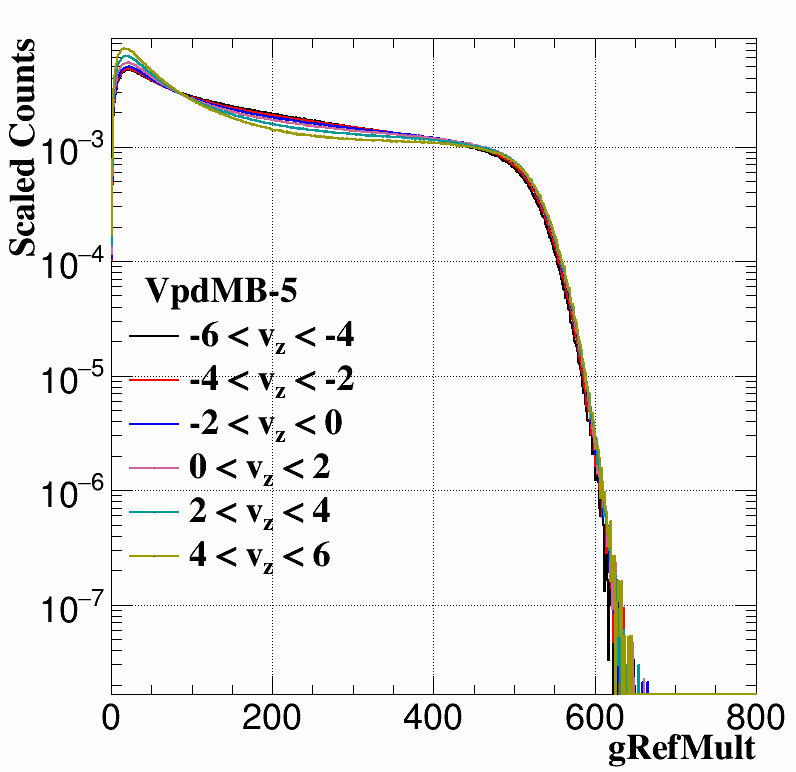
\includegraphics[width=0.75\textwidth]{fig/MB5_gref.png}
\caption{Normalized gRefmult distribution for VpdMB5 trigger along different $V_{z}$ range\label{fig:MB5_vz}}
\end{minipage}
\hfill
\begin{minipage}[htbp]{0.52\linewidth}
\centering
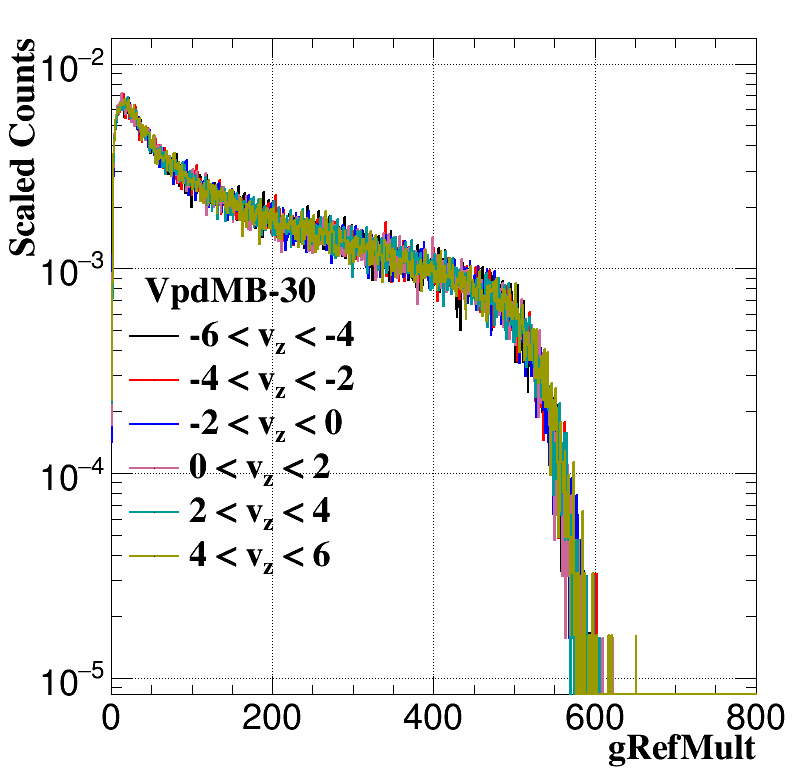
\includegraphics[width=0.75\textwidth]{fig/MB30_gref.png} 
\caption{Normalized gRefmult distribution for VpdMB30 trigger along different $V_{z}$ range\label{fig:MB30_vz}}
\end{minipage}
\end{figure}

As the gRefmult have the luminosity dependence (related to the TPC tracking efficiency have luminosity dependence), we need to take out this effect by doing ZdcX (Zdc coincidence rate) correction. Fig.~\ref{fig:MB5_zdc1} shows the mean value of gRefmult (<gRefmult>) distribution as a function of ZdcX. There was a clear slope for this distribution as shown by the fitting parameters. Here the fitting function is Eq.~\ref{funzdc},
\begin{equation}
f_{ZdcX} = p0 + p1*ZdcX
\label{funzdc}
\end{equation}
The goal of this correction is try to flatten this ZdcX dependence to take out of the luminosity effect. So here the correction factor was shown by  Eq.~\ref{funzdc2}.
\begin{equation}
f_{ZdcX} = \frac{1}{1 + p1/p0*ZdcX}
\label{funzdc2}
\end{equation}
After the ZdcX correction, this <gRefmult> is flat as shown by Fig.~\ref{fig:MB5_zdc2}.

For the $V_{z}$ dependence correction, we extract the high end point (h) from the fitting of gRefmult tail by the function of Eq.~\ref{funerf}.
\begin{equation}
f_{x} = A * TMath::Erf(-\sigma*(x-h)) + A
\label{funerf}
\end{equation}

\begin{figure}[htbp]
\begin{minipage}[htbp]{0.52\linewidth}
\centering
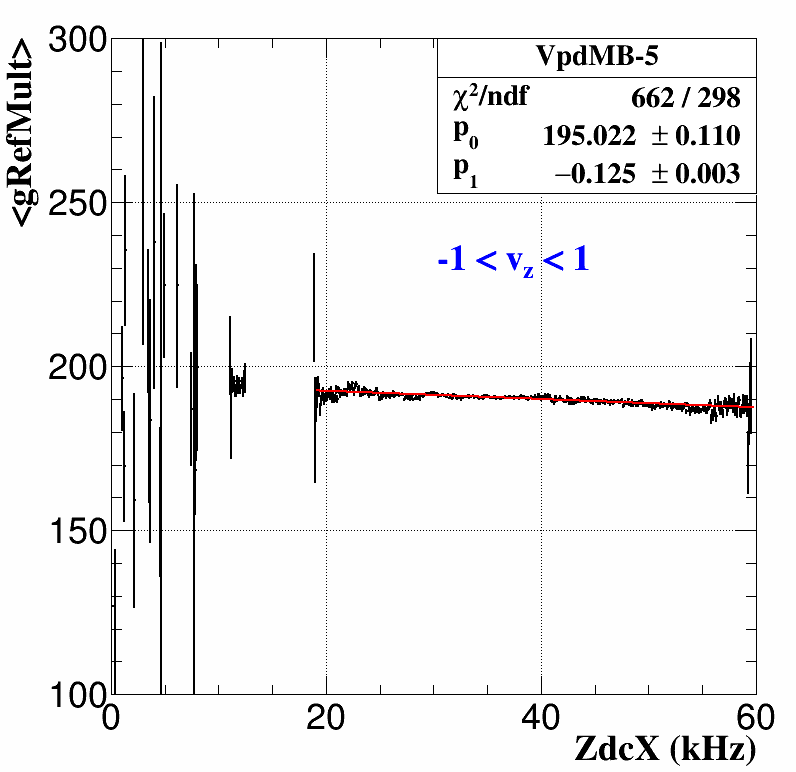
\includegraphics[width=0.75\textwidth]{fig/MB5_ZDCcor1.png}
\caption{<gRefmult> as function of ZdcX before correction.\label{fig:MB5_zdc1}}
\end{minipage}
\hfill
\begin{minipage}[htbp]{0.52\linewidth}
\centering
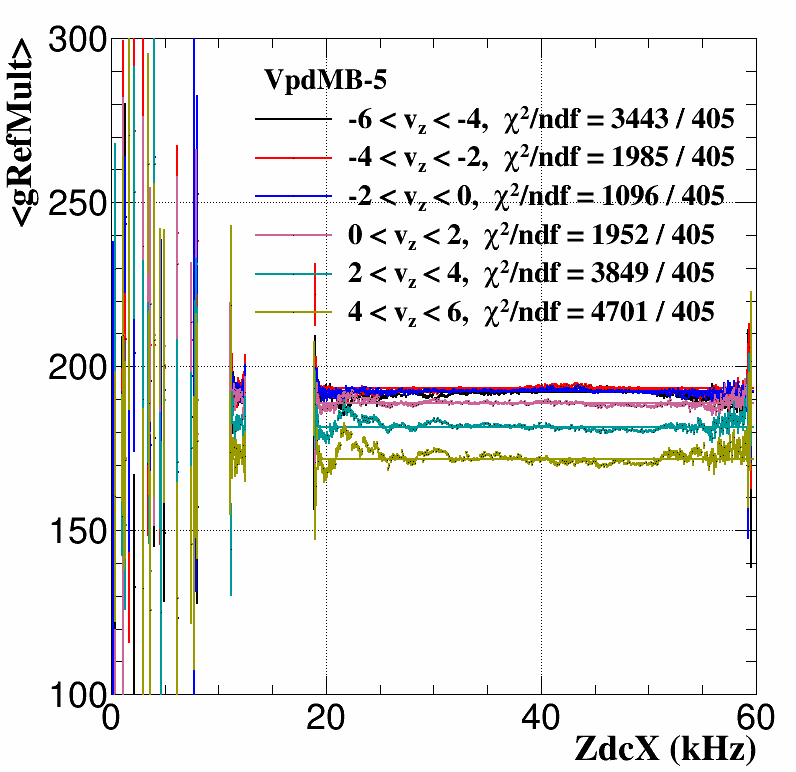
\includegraphics[width=0.75\textwidth]{fig/MB5_ZDCcor2.png} 
\caption{<gRefmult> as function of ZdcX after correction.\label{fig:MB5_zdc2}}
\end{minipage}
\end{figure}

Fig.~\ref{fig:MB5_vz1} shows an example of the fitting of gRefmult tail in the $V_{z}$ range from 1 cm to 2 cm. The fitting parameters were shown on the plot.

\begin{figure}[htbp]
\centering
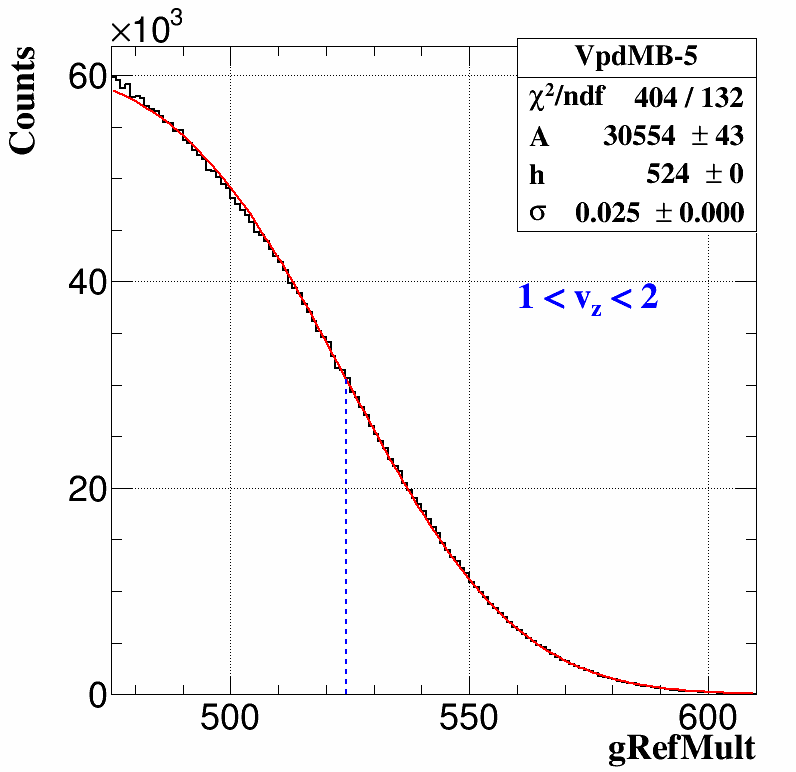
\includegraphics[keepaspectratio,width=0.5\textwidth]{fig/MB5_Vzcor1.png}
\caption{Fitting gRefmult tail distribution in the range of 1<$V_{z}$<2 cm by Eq.~\ref{funerf}.}
 \label{fig:MB5_vz1}
\end{figure}

With all the high end point value extracted along $V_{z}$ direction, this $V_{z}$ dependence was shown on Fig.~\ref{fig:MB5_vz2}. The similar method as ZdcX correction, we need to flatten this $V_{z}$ dependence, then the data point was fitted by 5th order polynomial function Eq.~\ref{funvz}, and then the correction factor was shown by Eq.~\ref{funvz2}
After the $V_{z}$ correction, this high end point is flat as shown by Fig.~\ref{fig:MB5_vz3}.

\begin{equation}
  f_{V_{z}} = p0 + p1*x + p2*x^2 + p3*x^3 + p4*x^4 + p5*x^5
\label{funvz}
\end{equation}

\begin{equation}
  f_{V_{z}} = \frac{p0}{p0 + p1*x + p2*x^2 + p3*x^3 + p4*x^4 + p5*x^5}
\label{funvz2}
\end{equation}


\begin{figure}[htbp]
\begin{minipage}[htbp]{0.52\linewidth}
\centering
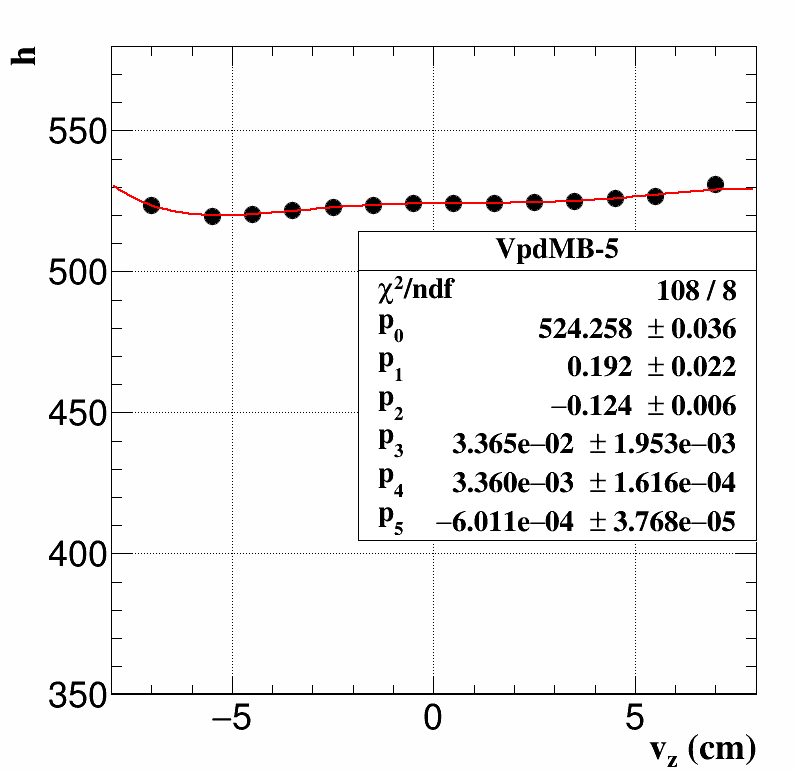
\includegraphics[width=0.75\textwidth]{fig/MB5_Vzcor2.png}
\caption{High end point as function of $V_{z}$ after correction.\label{fig:MB5_vz2}}
\end{minipage}
\hfill
\begin{minipage}[htbp]{0.52\linewidth}
\centering
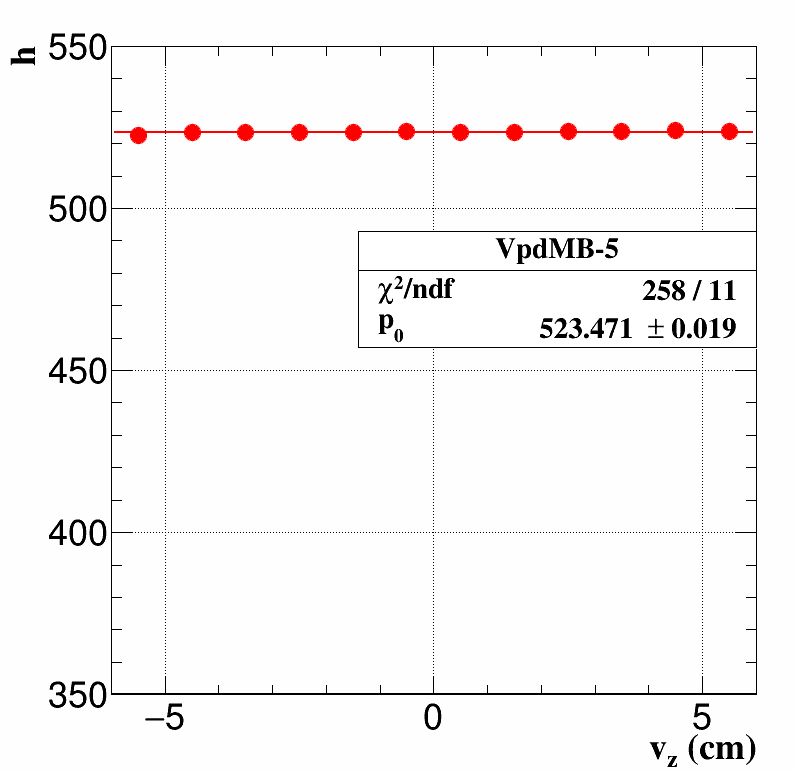
\includegraphics[width=0.75\textwidth]{fig/MB5_Vzcor3.png} 
\caption{High end point  as function of $V_{z}$ after correction.\label{fig:MB5_vz3}}
\end{minipage}
\end{figure}

As shown from Fig.~\ref{fig:MB5_vz} and Fig.~\ref{fig:MB30_vz}, the clear $V_{z}$ dependence need to avoid for VpdMB5 trigger. So, the centrality definition for VpdMB5 trigger was normalized to VpdMB30. After the ZdcX correction and $V_{z}$ correction, we directly take it as an additional correction factor for VpdMB5. These correction factor was show in Fig.~\ref{fig:MB5_vzscale}. After this additional correction, the distributions from VpdMB5 and VpdMB30 are same.

\begin{figure}[htbp]
\centering
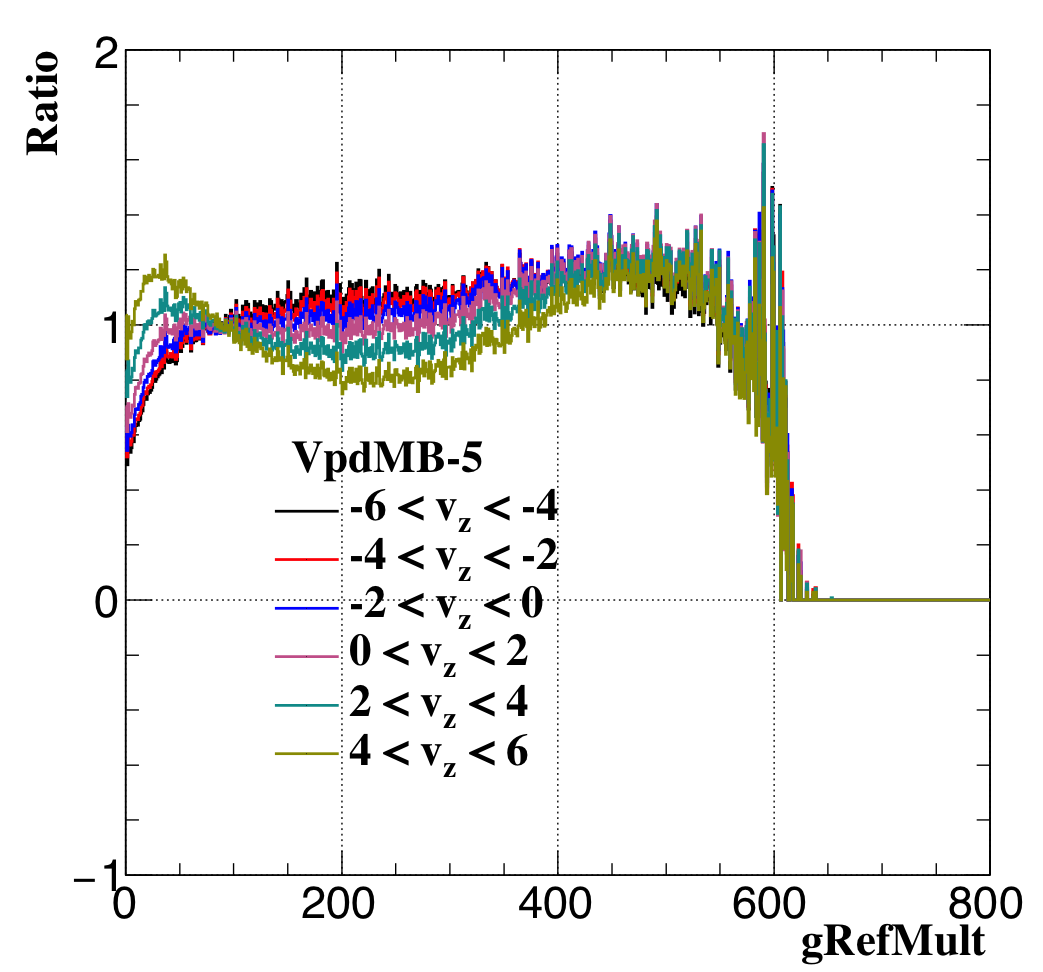
\includegraphics[keepaspectratio,width=0.5\textwidth]{fig/MB5_VzScale.png}
\caption{The double ratio of normalized gRefmult distribution from VpdMB5 over VpdMB30, this additional correction factor was try to normalized VpdMB5 to VpdMB30 trigger.}
 \label{fig:MB5_vzscale}
\end{figure}

The Vpd MinBias trigger has a trigger efficiency that are lower for periheral events. Fig.~\ref{fig:McData} shows the gRefmult after $V_{z}$ and ZdcX correction from data comparison with Glauber MC simulation. In the high end part the agreement was well, but in the low end part, due to this trigger ineffciency, there is clearly discrepancy between data and simulation. To do the measurement without centrality bias, a weight proportional to inverse trigger efficiency is applied. The weight as a function of corrected gRefMult is shown in Fig.~\ref{fig:vpdEffWeight}.

\begin{figure}[htbp]
\begin{minipage}[htbp]{0.52\linewidth}
\centering
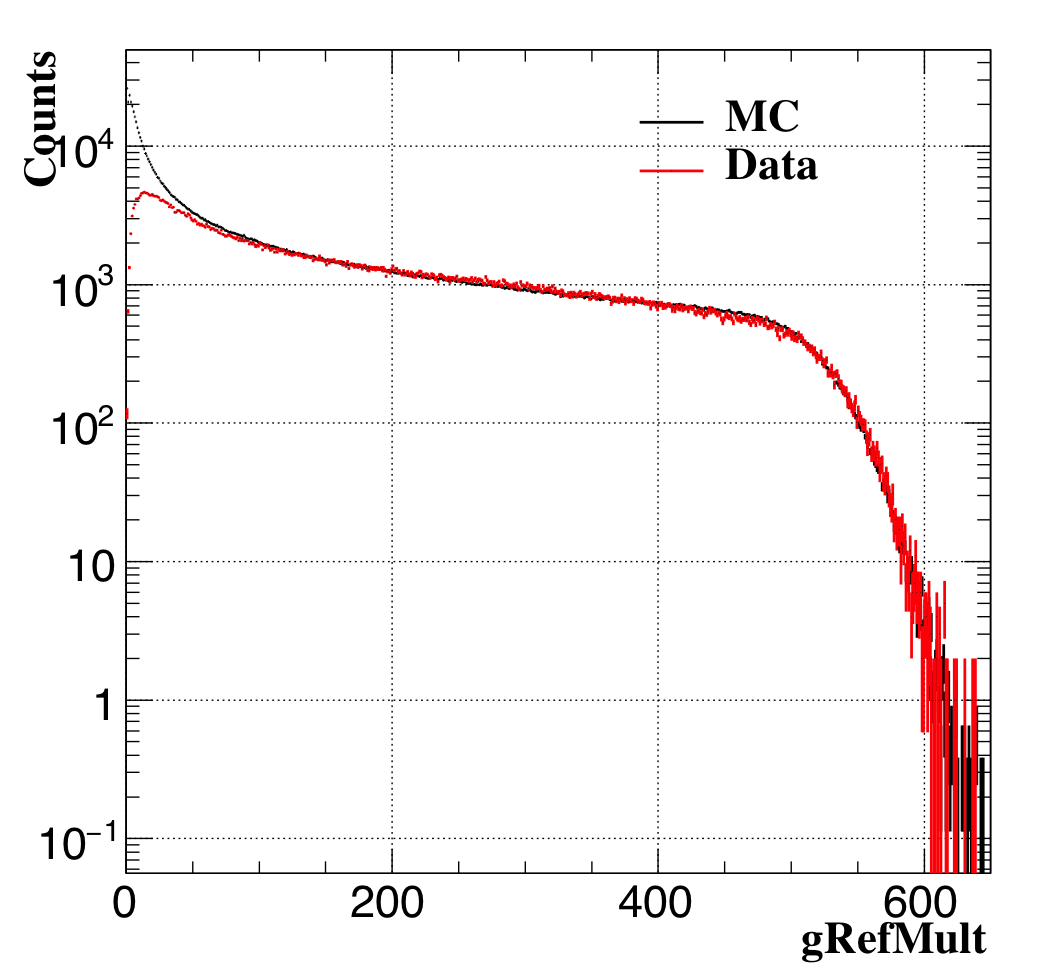
\includegraphics[width=0.75\textwidth]{fig/MB30_Mc_compare.png}
\caption{The comparison of corrected gRefMult between Data and Glauber MC. The red line is data and the black line is from Glauber MC.\label{fig:McData}}
\end{minipage}
\hfill
\begin{minipage}[htbp]{0.52\linewidth}
\centering
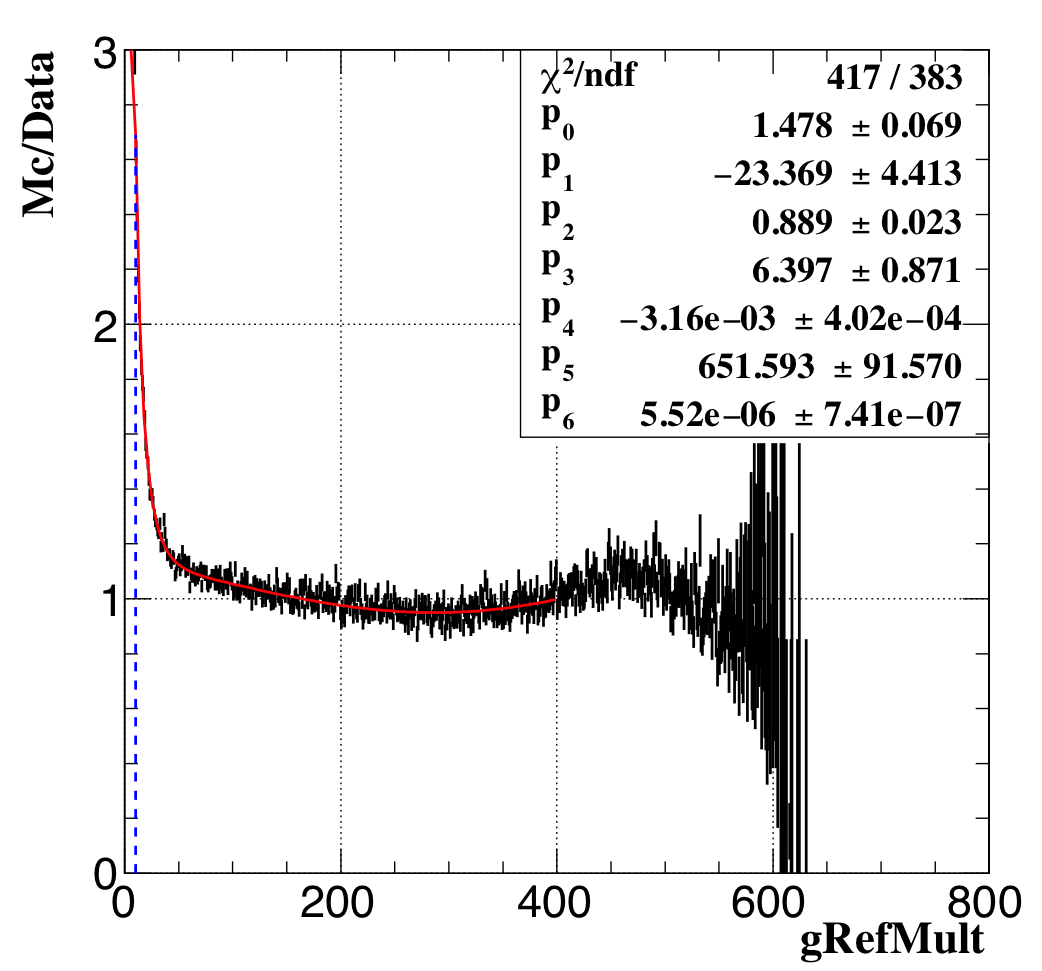
\includegraphics[width=0.75\textwidth]{fig/MB30_Mc_reweight.png} 
\caption{MC/data gRefmult distribution for Vpd MinBias trigger efficiency correction. The red line fit function is the correction reweight function.\label{fig:vpdEffWeight}}
\end{minipage}
\end{figure}

\begin{figure}[htbp]
\centering
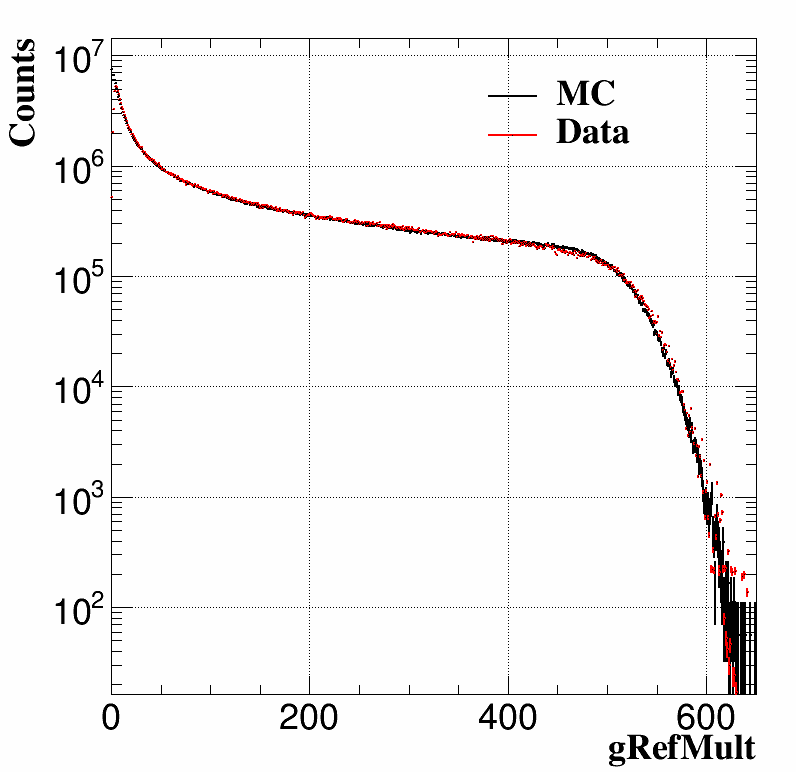
\includegraphics[keepaspectratio,width=0.5\textwidth]{fig/MB5_AfterALLMCData.png}
\caption{The comparison of corrected gRefMult (after all corrections and reweight) between Data and Glauber MC. The red line is data and the black line is from Glauber MC.\label{fig:MB5_afterAll}}
\end{figure}

After all these corrections including $V_{z}$, ZdcX, Vpd trigger inefficiency, and Vpd resolution for different centralities as discussed before. Final step, the data was compared to Glauber MC simulation as shown in Fig.~\ref{fig:MB5_afterAll}. And then the determined centrality classification can be found at Table ~\ref{centrality}.

\begin{table}[htp]
	\begin{center}
	\begin{tabular}{l|l|l|l}
  \toprule[1.6pt]
  \hline
  centrality & gRefMult & {$\langle$$N_{coll}$$\rangle$} & {$\langle$$N_{part}$$\rangle$} \\ \hline
  75-80$\%$ &	10-15	& 10.48 &	11.82 \\ \hline
	70-75$\%$ &	15-21	&	16.11 &	16.68 \\ \hline
	65-70$\%$ &	21-30	&	24.59 &	23.25 \\ \hline
	60-65$\%$ &	30-41	&	36.13 &	31.15 \\ \hline
	55-60$\%$ &	41-56	&	52.77 &	41.27 \\ \hline
	50-55$\%$ &	56-73	&	75.36 &	53.46 \\ \hline
  45-50$\%$ &	73-94	&	105.25 & 67.93 \\ \hline
  40-45$\%$ &	94-119 & 143.54 &	84.71 \\ \hline
  35-40$\%$ &	119-148	& 191.83 & 103.99 \\ \hline
	30-35$\%$ &	148-182	& 253.13 & 126.52 \\ \hline
	25-30$\%$ &	182-221	& 328.99 & 152.31 \\ \hline
	20-25$\%$ &	221-266	& 422.49 & 181.93 \\ \hline
	15-20$\%$ &	266-317	& 537.52 & 215.98 \\ \hline
	10-15$\%$ &	317-376	& 677.99 & 254.90 \\ \hline
	5-10 $\%$ &	376-443	& 852.75 & 299.95 \\ \hline
  0-5	 $\%$	& $>$443	& 1066.50	& 348.74 \\ \hline
  \hline
  \bottomrule[1.6pt]
	\end{tabular}
	\caption{Centrality defintion based on gRefMult}
	\label{centrality}
	\end{center}
\end{table}

\section{$D^0$ Reconstruction}

$D^{0}$ and $\bar{D^{0}}$ are reconstructed through the typically hadronic channel $K^{\mp}\pi^{\pm}$ using the topological method. In the following we will describe the daughter selection, the geometry cuts and how they are obtained through the TMVA tuning. We will show the $D^0$ signals for different $p_T$ bins. We will also discuss some related topics: the mixed event to reconstruct the combinatorial background, and the correlated background source shown as a `bump' at invariant mass lower than the $D^0$. 

\subsection{Daughter Selection}
\label{daughterSelection}
$D^0$ have a lifetime of $c\tau\sim123 \upmu$m. Thus the global tracks for daughter tracks are used in this analysis. The transverse momentum are required to $\geq$ 0.3 GeV/$c$ to ensure that the track can pass through the TPC and have less HFT miss matching, the number of hit points (nHits) along the track is $\geq$ 20 (of a maximum of 45) to ensure good momentum resolution.

The pion and kaon tracks are identified by combining Time Projection Chamber (TPC) and Time Of Flight detector (TOF). The TPC provides particle identification utilizing the energy loss information $dE/dx$, different particle species with the same momentum may have different $dE/dx$. In additional, different particle species with the same momentum have different velocities, thus the TOF can be used to identify different particle species in the $dE/dx$ crossover regions by precise velocity information ($1/\beta$ = $ct/l$). The normalized $dE/dx$, $n\sigma_x$ (x = $\pi$, K, p, e etc.), defined in Eq.~\ref{nsigma}, instead of $dE/dx$ is used in this analysis. Where $\langle{dE/dx}\rangle_{measured}$ and $\langle{dE/dx}\rangle_{x}$ represent measured and theoretical $dE/dx$, and $R$ is the STAR TPC $dE/dx$ resolution (typically $\sim$8\%). The $n\sigma_x$ should be close to a standard Gaussian distribution for each corresponding particle species (mean $=$ 0, $\sigma = $ 1).
\begin{equation}
  n\sigma_x = \frac{1}{R}log\frac{\langle{dE/dx}\rangle_{measured}}{\langle{dE/dx}\rangle_{x}}
\label{nsigma}
\end{equation}

Fig.~\ref{fig:tpcPID} shows the TPC energy loss dE/dx information versus momentum achieved from Run14 Au+Au 200GeV, there are several clear bands for different particle species such as $\pi$, K, p and e. 

Fig.~\ref{fig:tofPID} shows the TOF 1/Beta information versus momentum achieved from Run14 Au+Au 200GeV, also there are several clear bands for different particle species such as $\pi$, K, p . 

\begin{figure}[htbp]
\centering
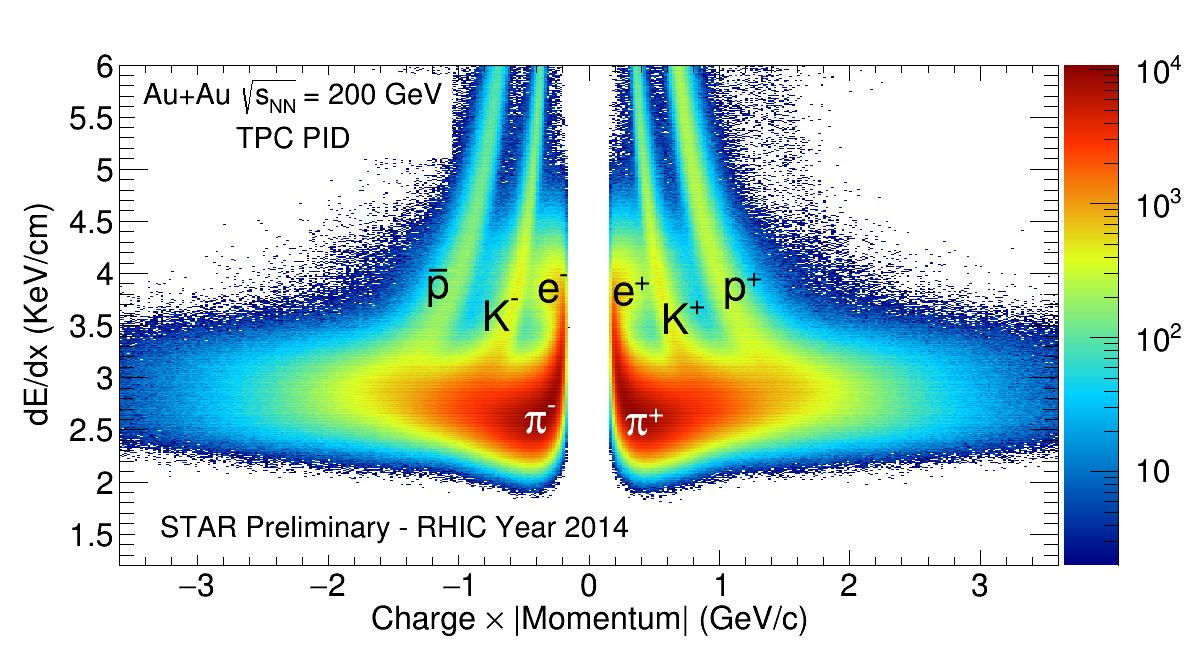
\includegraphics[keepaspectratio,width=0.8\textwidth]{fig/Run14_AuAu_dEdx_PR_copy.png}
\caption{TPC dE/dx versus charge$\times$momentum achieved from Run14 Au+Au 200GeV.}
 \label{fig:tpcPID}
\end{figure}

\begin{figure}[htbp]
\centering
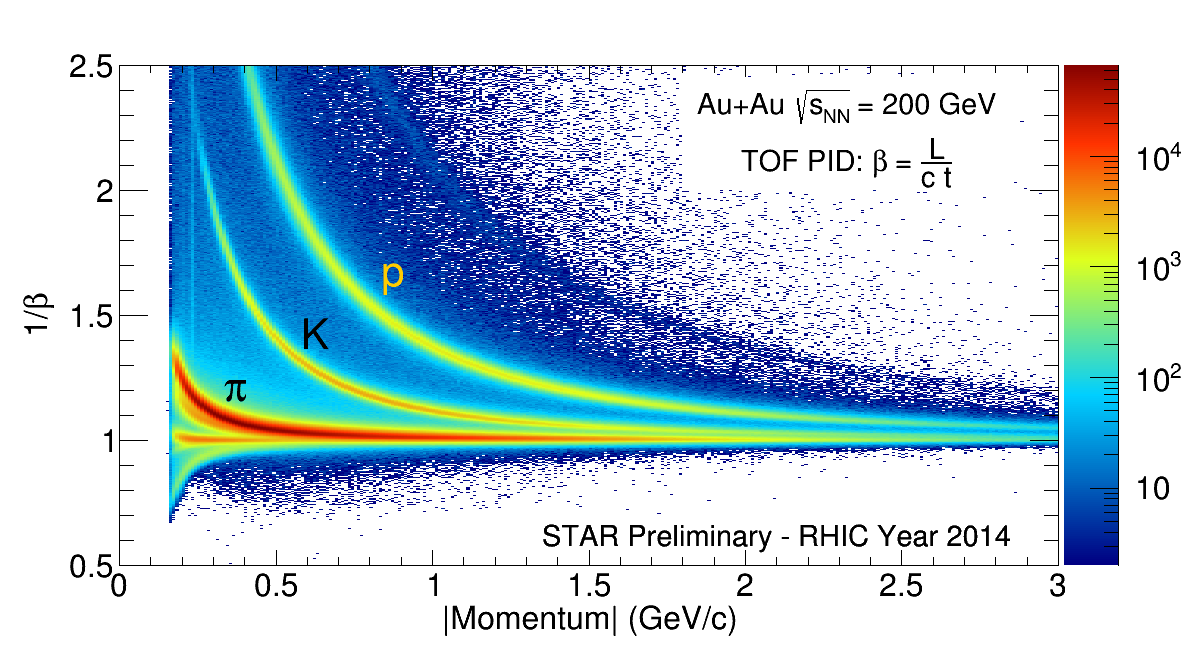
\includegraphics[keepaspectratio,width=0.8\textwidth]{fig/Run14_AuAu_tofBeta_PR.png}
\caption{TOF 1/Beta versus momentum achieved from Run14 Au+Au 200GeV.}
 \label{fig:tofPID}
\end{figure}

In summary, next list all the related track selections for $D^0$ daughters including track quality cut and particle identification cut.
\begin{itemize}
\item global tracks
\item $p_{T}$ > 0.3 GeV/$c$
\item $|\eta| < 1$
\item $nHitsFit \ge 20$, in TPC
\item at least one hit in every layer of PXL and IST
\end{itemize}

pion PID:
\begin{itemize}
  \item $|n\sigma_{\pi}| < 3.0 $, based on TPC dE/dx
  \item If TOF is avaliable (hybrid PID):  $|\frac{1}{\beta}-\frac{1}{\beta_{exp}}|<0.03$
\end{itemize}

kaon PID:
\begin{itemize}
  \item $|n\sigma_{K}| < 2.0 $, based on TPC dE/dx
  \item If TOF is avaliable (hybrid PID):  $|\frac{1}{\beta}-\frac{1}{\beta_{exp}}|<0.03$
\end{itemize}


\subsection{Topological Cut Optimization}

The secondary vertex is reconstructed with selected kaon and pion global tracks. In this analysis, the middle point on the Distance of the Closest Approach (DCA) between two daughter tracks is considered as the secondary decay vertex of the candidate $D^0$. As shown in Fig.~\ref{fig:D0cartoon}, 5 geometrical variables are chosen to select $D^0$ and reject combinatorial background, which is dominated by a pair of tracks directly from the primary vertex: decay length (the distance between the decay vertex and Primary Vertex PV), DCA between the 2 daughters, DCA between the reconstructed $D^0$ flying path and PV, DCA between the $\pi$ track and PV, and DCA between the $K$ track and PV. The cuts on these variables are optimized by the Toolkit for Multivariate Data Analysis (TMVA) package. They change according to the $D^0$ candidate $p_T$ in order to have the best significance in all the covered $p_T$ range. Additionally there is a $cos(\theta) > 0$ cut to make sure the decay vertex with respect to the primary vertex is roughly in the same direction as the momentum.

\begin{figure}[htbp]
\centering
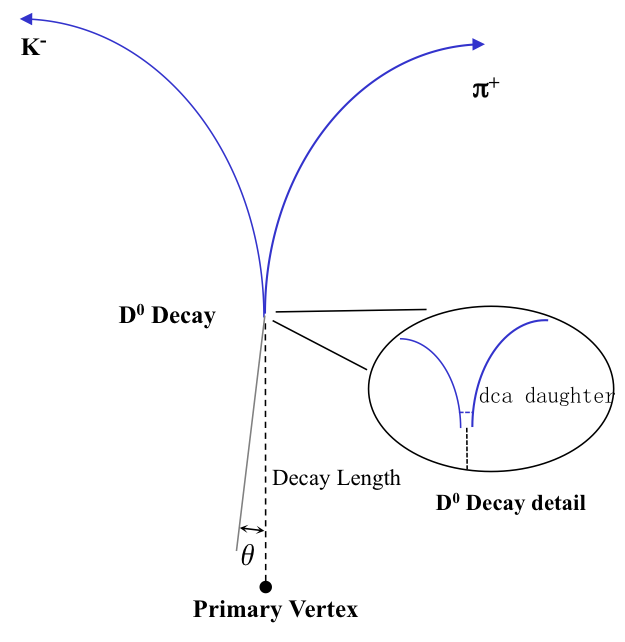
\includegraphics[keepaspectratio,width=0.6\textwidth]{fig/D0cartoon.png}
\caption{The topology of a $D^0$ decaying to a kaon and a pion.}
 \label{fig:D0cartoon}
\end{figure}

The TMVA need signal and background sample input for training. The signal sample is obtained from a toy fast-simulation and the background sample is from real data like sign pairs in $D^0$ mass window and unlike sign pairs in side bands range. 

Fig.~\ref{fig:variables} shows distributions of the 5 geometry variables for signal (blue) and background (red) plotted by the TMVA, for $p_T$ between 2 and 3 GeV/$c$.

\begin{figure}[htbp]
\centering
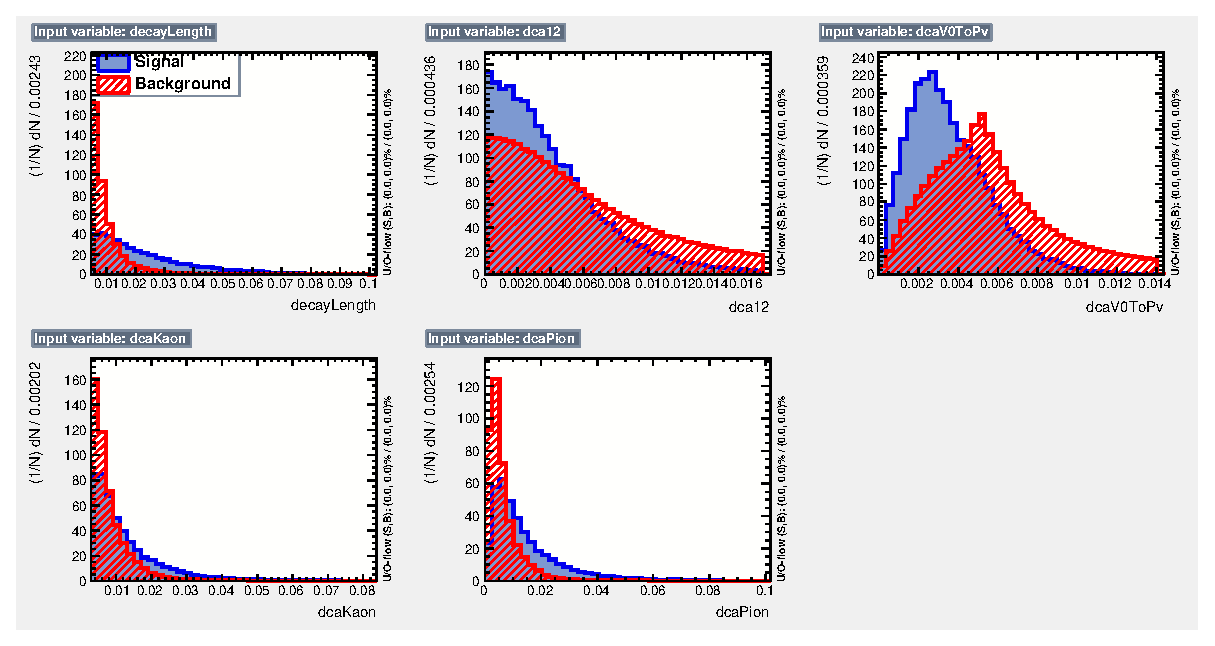
\includegraphics[keepaspectratio,width=1.0\textwidth]{fig/variables_id_c1.eps}
\figcaption{Distributions of the 5 geometry variables for signal (blue) and background (red).}
\label{fig:variables}
\end{figure}

The `cuts' option of TMVA is used to tune $D^0$ cuts. This option randomly sample different cut sets in the variable space, calculate signal and background efficiency for each cut set. Then one cut set with lowest background efficiency at certain signal efficiency. We can then pick the cut set with the best significance according to the signal and background yield corresponding to the whole data set. Fig.~\ref{fig:effPass4} shows the lowest background efficiency, significance and so on vs. signal efficiency for $p_T$ between 2 and 3 GeV/$c$. We can see that as cuts get tighter, signal and background efficiency both decrease, but background efficiency decreases much faster.

\begin{figure}[htbp]
\centering
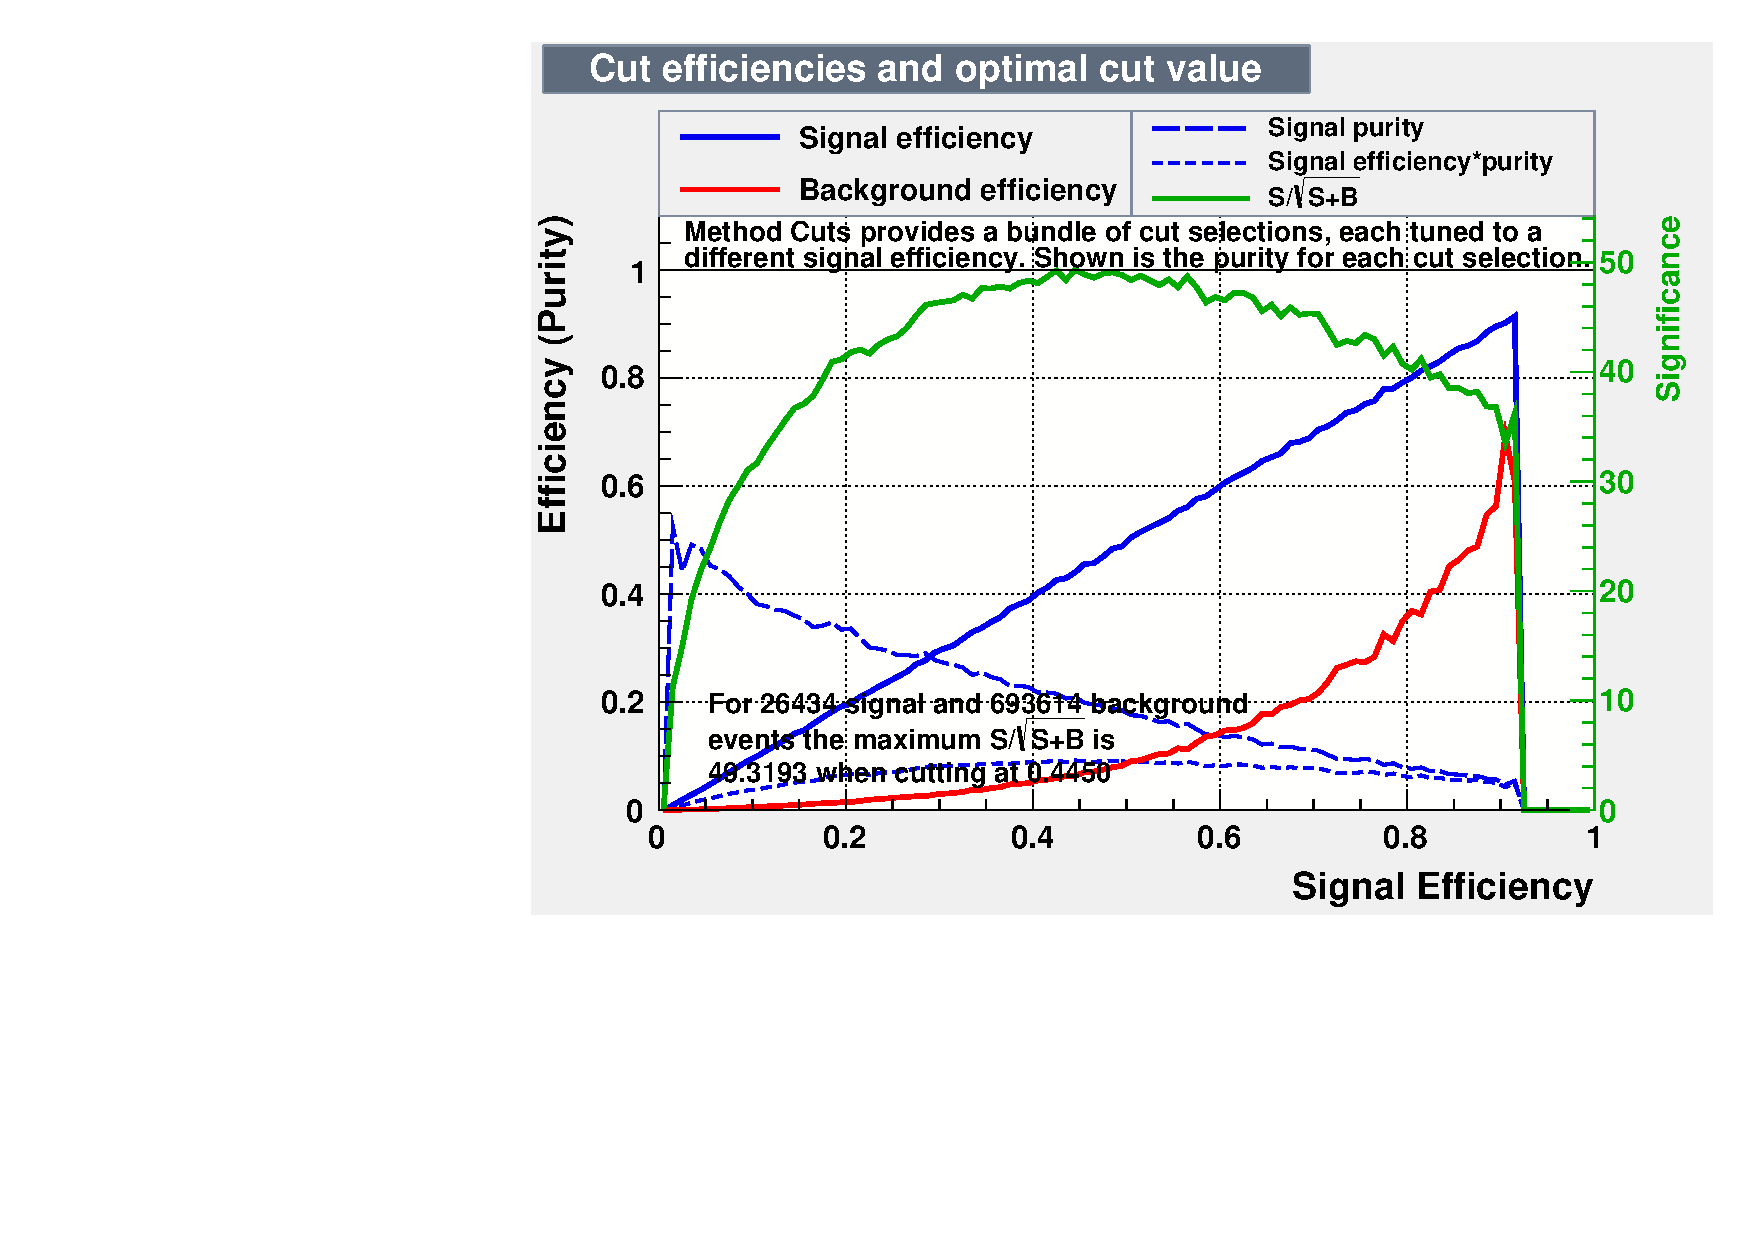
\includegraphics[keepaspectratio,width=0.5\textwidth,angle=0]{fig/effPass4.pdf}
\figcaption{Signal efficiency, lowest background efficiency, significance and so on vs. signal efficiency.}
\label{fig:effPass4}
\end{figure}

\begin{table}[htp]
  \centering
  \caption{Standard geometrical cuts for different $D^0$ $p_T$.}
  \label{geometryCuts}
  \begin{center}
    \begin{tabular}{l|l|l|l|l|l}
      % \Xhline{1.6pt}
      $D^0$ $p_T$ (GeV/$c$) & 0-1 & 1-2 & 2-3 & 3-5 & 5-10\\ \hline
      decay length (${\upmu}m$) $>$ & 145 & 181 & 212 & 247 & 259\\ \hline
      DCA between 2 daughters (${\upmu}m$) $<$ & 84 & 66 & 57 & 50 & 60\\ \hline
      DCA between $D^0$ and PV (${\upmu}m$) $<$ & 61 & 49 & 38 & 38 & 40\\ \hline
      DCA between $\pi$ and PV (${\upmu}m$) $>$ & 110 & 111 & 86 & 81 & 62\\ \hline
      DCA between $K$ and PV (${\upmu}m$) $>$ & 103 & 91 & 95 & 79 & 58\\ \hline
      % \Xhline{1.6pt}
    \end{tabular}
  \end{center}
\end{table}

\begin{table}[htp]
  \centering
  \caption{Tight geometrical cuts for different $D^0$ $p_T$.}
  \label{geometryCutsTight}
  \begin{center}
    \begin{tabular}{l|l|l|l|l|l}
      % \Xhline{1.6pt}
      $D^0$ $p_T$ (GeV/$c$) & 0-1 & 1-2 & 2-3 & 3-5 & 5-10\\ \hline
      decay length (${\upmu}m$) $>$ & 144 & 204 & 242 & 245 & 300\\\hline
      DCA between 2 daughters (${\upmu}m$) $<$ & 69 & 48 & 44 & 49 & 47\\ \hline
      DCA between $D^0$ and PV (${\upmu}m$) $<$ & 44 & 36 & 31 & 26 & 32\\ \hline
      DCA between $\pi$ and PV (${\upmu}m$) $>$ & 120 & 102 & 118 & 109 & 96\\ \hline
      DCA between $K$ and PV (${\upmu}m$) $>$ & 119 & 110 & 109 & 106 & 80\\ \hline
      % \Xhline{1.6pt}
    \end{tabular}
  \end{center}
\end{table}


\begin{table}[htp]
  \centering
  \caption{Loose geometrical cuts for different $D^0$ $p_T$.}
  \label{geometryCutsLoose}
  \begin{center}
    \begin{tabular}{l|l|l|l|l|l}
      % \Xhline{1.6pt}
      $D^0$ $p_T$ (GeV/$c$) & 0-1 & 1-2 & 2-3 & 3-5 & 5-10\\ \hline
      decay length (${\upmu}m$) $>$ & 110 & 168 & 187 & 199 & 180\\ \hline
      DCA between 2 daughters (${\upmu}m$) $<$ & 77 & 78 & 74 & 68 & 66\\ \hline
      DCA between $D^0$ and PV (${\upmu}m$) $<$ & 72 & 53 & 47 & 42 & 62\\ \hline
      DCA between $\pi$ and PV (${\upmu}m$) $>$ & 92 & 78 & 86 & 65 & 47\\ \hline
      DCA between $K$ and PV (${\upmu}m$) $>$ & 105 & 68 & 80 & 66 & 41\\ \hline
      % \Xhline{1.6pt}
    \end{tabular}
  \end{center}
\end{table}

The result of the geometry cuts tuned for best significance are shown in Table \ref{geometryCuts}. These are the standard cuts used in the $D^0$ reconstruction to calculate the spectra central value.

For $D^0$ estimation, another 2 sets of geometry cuts are tuned with TMVA, with 50\% and 150\% signal efficiency relative to the standard cuts. They do not give the overall best $D^0$ significance, but for the certain signal efficiency, they are still the cuts with the lowest background efficiency and best $D^0$ significance. With 50\% and 150\% signal efficiency relative to the standard cuts, their significance is still about 80\% of the standard cuts with the overall best significance. These 2 cuts sets are listed in Table \ref{geometryCutsTight} and \ref{geometryCutsLoose}.

For more details can be found in the $D^0$ $v_2$ technicl note, basically we use the same cuts for spectra analysis and $v_2$ analysis.

\subsection{Mixed Event Background}

To construct the mixed event background it is important to combine events with some degree of similarity, such as events are classified according to the position of the primary vertex (PV) along the beam-line, the centrality class and the orientation of the event plane. Ten bins of equal width were used for both the event plane ($\Psi\in[-\pi,\pi]$) and the position of the primary vertex($V_z\in[-6,6]$), as well as nine centrality classes between 0-80\%, for a total of 900 event `categories'.

Table \ref{eventBuf} summarizes the important information saved for the event mixing:

\begin{table}[htp]
\centering
\caption{Summary of information saved for the event mixing}
\label{eventBuf}
\begin{tabular}{ l | l  }
\toprule[1.6pt]
StMixerTrack & StMixerEvent \\
\midrule[1.2pt]
Origin & PV Origin \\
\\
Momentum & Magnetic Field \\
\\
Q-Vector & Event Plane \\
\\
Track information & Array of mixer tracks \\
\\
  &Array of indices to identified pions \\
\\
  & Array of indices to identified kaons \\
\\
\bottomrule[1.6pt]
\end{tabular}
\end{table}

For the more details of the mixed-event backgrounds and the `bump' structures in the foreground, they also can be found in the $v_2$ analysis note.

\subsection{Correlated background `bump' for $D^0$ meson}

\section{Efficiency Correction}
General idea.....

\subsection{TPC Tracking Efficiency}

\subsection{Data-driven fast Monte Carlo setup for HFT and Topological Cut Efficiency}

\subsection{Validation with Full GEANT+Hijing Simulation}

\subsection{PID Efficiency and Double Counting Correction}

The PID efficiency part includes the efficiency from $dE/dx$ or $n\sigma$ cut efficiency and the TOF matching+$1/\beta$ cut efficiency. The $dE/dx$ and $1/\beta$ calibration usually uses a specific set of tracks. The performance for identified particles that pass our analysis cut may not necessarily be exactly normal Gaussian distributions with means=0 and widths=1. It is desired to calibrate each individual distributions for identified particles for efficiency correction and mis-PID effect study.

For $n\sigma$ calibration, we followed the same method as described in Ref.~\cite{Xu:2008th} to calibrate high $p_{\rm T}$ pions and protons by selecting daughters from $K_{S}^0$ and $\Lambda$ decays.

\subsubsection{$dE/dx$ Calibration}



\subsection{Vertex Resolution Correction}

\subsection{Validation with Ks Spectra Measurement}

\begin{figure}
\centering
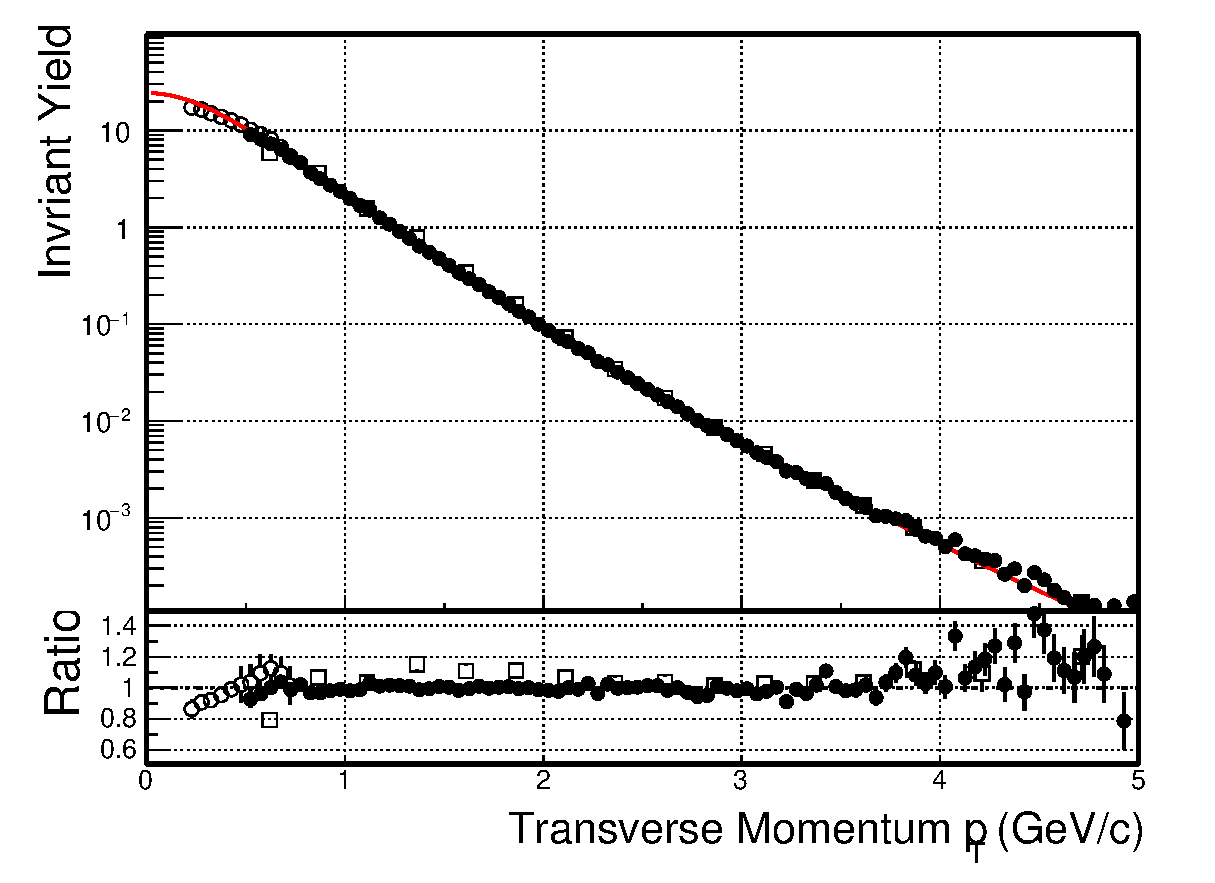
\includegraphics[width=0.7\textwidth]{fig/Ks_spectra_PtCut_0.eps}
\caption{\label{fig:Ks_spectra}Ks spectra.}
\end{figure}

\section{\label{results}Results}

\section{\label{Run1011}Re-analysis of Run10/11 data}

\subsection{Long and Yifei's re-analysis}

\subsection{Xiaolong's re-analysis}

\section{\label{Run14TPC}Run14 TPC analysis}

\bibliographystyle{alpha}
\bibliography{D0spectra_Note}

\end{document}
